% SecureNWDAF -- free5GC Forum 2026 long-paper draft
% IMPORTANT: This draft intentionally contains NO results from the previous
% 90/120/80-run campaigns. Replace every [TBD] result after the new campaign.
%
% Compile:
%   pdflatex SecureNWDAF_free5GC_Forum2026_12page_draft.tex
%   pdflatex SecureNWDAF_free5GC_Forum2026_12page_draft.tex

\documentclass[sigconf,review]{acmart}

\settopmatter{printacmref=true,printfolios=true}
\renewcommand\footnotetextcopyrightpermission[1]{}
\pagestyle{plain}

\usepackage{booktabs}
\usepackage{multirow}
\usepackage{amsmath}
\usepackage{graphicx}
\usepackage{xcolor}
\usepackage{tikz}
\usetikzlibrary{arrows.meta,positioning,shapes.geometric,fit,calc,backgrounds}
\usepackage{pgfplots}
\pgfplotsset{compat=1.18}
\usepackage{enumitem}
\usepackage{balance}
\usepackage{tabularx}
\usepackage{array}
\usepackage{placeins}
\usepackage{url}
\usepackage{microtype}

\setlength{\emergencystretch}{3em}
\sloppy
\raggedbottom

% Restrained academic palette.
\definecolor{coreblue}{HTML}{2B5D8A}
\definecolor{securityred}{HTML}{8A3B3B}
\definecolor{softgray}{HTML}{F3F5F7}
\definecolor{softgreen}{HTML}{EEF5F0}

\tikzset{
  box/.style={draw=coreblue,rounded corners=2pt,fill=blue!3,align=center,font=\footnotesize,minimum height=7mm,minimum width=25mm},
  secbox/.style={draw=securityred,rounded corners=2pt,fill=red!3,align=center,font=\footnotesize,minimum height=7mm,minimum width=25mm},
  data/.style={draw=black!55,rounded corners=2pt,fill=black!2,align=center,font=\footnotesize,minimum height=7mm,minimum width=25mm},
  decision/.style={diamond,draw=securityred,fill=red!3,align=center,font=\scriptsize,aspect=1.55,inner sep=1pt},
  arrow/.style={-{Latex[length=1.8mm]},semithick,draw=coreblue},
  secarrow/.style={-{Latex[length=1.8mm]},semithick,draw=securityred},
  dasharrow/.style={-{Latex[length=1.8mm]},semithick,dashed,draw=black!60}
}

% New-campaign placeholders. DO NOT submit until replaced.
\newcommand{\TBD}{\textbf{[TBD]}}
\newcommand{\newruns}{\TBD}
\newcommand{\testruns}{\TBD}
\newcommand{\RFPrecision}{\TBD}
\newcommand{\RFRecall}{\TBD}
\newcommand{\RFFOne}{\TBD}
\newcommand{\RFFPR}{\TBD}
\newcommand{\BZeroFone}{\TBD}
\newcommand{\MLPFOne}{\TBD}
\newcommand{\GRUFOne}{\TBD}
\newcommand{\DetLat}{\TBD}
\newcommand{\RespLat}{\TBD}
\newcommand{\ApplyRate}{\TBD}
\newcommand{\RestoreRate}{\TBD}
\newcommand{\FalseAction}{\TBD}
\newcommand{\CPUOverhead}{\TBD}
\newcommand{\TelemetryOverhead}{\TBD}

\begin{document}

\title{SecureNWDAF: Cross-Layer Security Analytics and Policy-Bounded Response for free5GC 5G Core Networks}

\author{Haochen Qin}
\affiliation{\institution{Nanyang Technological University}\city{Singapore}\country{Singapore}}
\email{QINH0007@e.ntu.edu.sg}

\author{Chee Wei Tan}
\affiliation{\institution{Nanyang Technological University}\city{Singapore}\country{Singapore}}
\email{cheewei.tan@ntu.edu.sg}

\begin{abstract}
Open-source 5G Core networks expose a security boundary that spans standardized network procedures and the Linux infrastructure on which network functions execute. Conventional network-only monitoring can miss host-level precursors, while unrestricted AI-driven automation creates a second risk: a model prediction can become an operational action without an explicit authorization boundary. This paper presents SecureNWDAF, a free5GC-based security analytics architecture that separates evidence collection, cross-layer correlation, anomaly diagnosis, policy evaluation, response execution, and verification. The design uses Network Data Analytics Function (NWDAF) terminology as a standards reference point while explicitly treating the implementation as an external research prototype rather than a full 3GPP NWDAF implementation. A two-machine testbed keeps the actual free5GC system on an Ubuntu host and places analytics, model management, evidence storage, and policy services on a separate GPU server. The experimental methodology is designed around run-level provenance and leakage-safe splits, controlled attack stimuli, multiple background loads, modality ablations, unseen-stimulus evaluation, online latency measurements, and paired response trials. A Random Forest is used as the primary detector because its behavior is inspectable and compatible with heterogeneous run-level features; optional neural backends are evaluated under the same split discipline. The response layer accepts only typed, authenticated, allow-listed, reversible actions after policy validation and post-condition checks. The new campaign is intended to quantify detection quality, generalization, analysis latency, enforcement latency, service impact, and system overhead without conflating detector accuracy with response success. Numerical results are intentionally left to the reproducible campaign described in this paper and are not inherited from earlier pilot datasets. The resulting framework provides a concrete experimental path for policy-bounded security analytics on free5GC and a cautious extension point toward future 6G non-terrestrial network environments.
\end{abstract}

\keywords{NWDAF, free5GC, 5G security, Linux security, anomaly detection, eBPF, policy enforcement, autonomous response, network resilience}

\ccsdesc[500]{Security and privacy~Network security}
\ccsdesc[300]{Networks~Mobile networks}
\ccsdesc[300]{Computing methodologies~Machine learning}
\ccsdesc[200]{Computer systems organization~Cloud computing}

\maketitle

\section{Introduction}
5G Standalone (SA) networks are increasingly implemented as software-defined systems whose network functions (NFs) execute on general-purpose computing platforms. The resulting architecture creates a useful convergence of networking and systems security: an AMF, SMF, UPF, or supporting service may be healthy at the protocol level while the Linux process environment, namespace boundary, routing state, or host resource condition is already abnormal. free5GC is an open-source 5G Core implementation designed for experimental and development use, supports the 3GPP service-based architecture (SBA), and is distributed with documentation for both standalone operation and simulated RAN/UE integration~\cite{free5gc,free5gcdocs}. The platform therefore provides a practical basis for evaluating security analytics on a real 5G software stack rather than on an abstract network simulator.

The security problem is not limited to malformed 5G messages. A lower-trust component may cause suspicious process creation, namespace transitions, runtime-socket access, capability changes, network-rule manipulation, resource exhaustion, or protocol anomalies. These signals have different meanings depending on workload identity, NF lifecycle, current service state, and the network effects that follow them. A process-level event alone may be benign during startup; the same event combined with an unexpected namespace target and subsequent service degradation may be a meaningful precursor. This motivates correlation across system, network, protocol, and service layers rather than treating a single log line as a verdict.

NWDAF is a natural architectural anchor for this problem because 3GPP defines it as a network analytics capability that can obtain data from authorized producers and provide analytics to authorized consumers. TS~23.288 defines the 5G architecture enhancements for network data analytics, while TS~29.520 specifies the NWDAF service-based interface~\cite{ts23288,ts29520}. Existing research has already explored abnormal-traffic analytics with NWDAF and machine learning, including microservice-based implementations and anomaly detectors evaluated with real 5G network data~\cite{yuan2022,mlnwdaf,oliveira2024}. However, the security boundary becomes less clear when an analytics output is connected directly to an operational action. A highly accurate detector is not, by itself, an authorization mechanism.

This paper therefore investigates a narrower and more systems-oriented question: \emph{can cross-layer security evidence be connected to policy-bounded operational response on free5GC without granting the analytics model direct authority over the network?} SecureNWDAF addresses this question with a modular design. DCCF-style processing normalizes and correlates evidence; an AnLF-style analyzer produces an evidence-backed diagnosis; a model registry maintains approved artifacts; an evidence store preserves provenance; a SecIR layer compiles typed response workflows; a policy decision point (PDP) checks action constraints; and an authenticated response agent performs only an allow-listed operation. The design treats the distinction between ``what the model believes'' and ``what the system permits'' as an explicit trust boundary.

The paper makes four concrete contributions. First, it defines a cross-layer security analytics architecture for free5GC that combines run-level Linux/process evidence with optional 5G protocol and service observations while preserving provenance and modality availability. Second, it implements a two-machine pipeline that keeps the actual free5GC environment independent from the GPU-side analytics stack, reflecting the practical separation used in the research testbed. Third, it defines a leakage-safe experimental protocol that uses run-level grouping, repeated controlled stimuli, load variation, modality ablations, unseen-stimulus tests, latency measurement, and paired response validation. Fourth, it implements a bounded response path in which a prediction is insufficient for execution: the action must satisfy explicit policy predicates, reach an authenticated adapter, produce a verifiable state transition, and remain reversible.

The paper asks three research questions:
\begin{enumerate}[leftmargin=*]
\item \textbf{RQ1:} How much does cross-layer run-level telemetry improve controlled anomaly detection relative to a simple load-based baseline under multiple operating loads?
\item \textbf{RQ2:} Which telemetry modalities contribute to detection and generalization, and can models retain performance on unseen stimulus seeds or operating conditions without event-level leakage?
\item \textbf{RQ3:} Can an evidence-backed diagnosis be converted into a bounded, authenticated, reversible response with measurable enforcement and restoration behavior while keeping operational authority outside the model?
\end{enumerate}

The rest of the paper is organized as follows. Section~2 summarizes the standards and related work. Section~3 defines the security problem and design goals. Section~4 presents the architecture. Section~5 describes the implementation. Section~6 defines the threat model and scenario taxonomy. Section~7 specifies the new experimental campaign. Section~8 defines the evaluation protocol and result reporting. Section~9 discusses security and systems implications. Section~10 covers limitations and the extension toward 6G NTN. Section~11 concludes the paper.

\section{Background and Related Work}
\subsection{NWDAF and 5G analytics}
3GPP TS~23.288 defines the architectural framework for network data analytics services in 5GS and describes responsibilities associated with data collection, analytics, and model management~\cite{ts23288}. TS~29.520 complements the architecture with the stage-3 service-based interface specification for NWDAF~\cite{ts29520}. These specifications provide an important semantic vocabulary for SecureNWDAF: analytics should be tied to authorized data producers and consumers, and analytics generation should remain conceptually separate from arbitrary network administration.

Research implementations demonstrate that an analytics framework can be integrated with a 5G core and used for anomaly detection. Mekrache et al. combine NWDAF and machine learning using an LSTM autoencoder and evaluate abnormal traffic using a 5G core environment~\cite{mlnwdaf}. Oliveira et al. describe a 5G core data analytics framework intended to simplify the development and integration of cybersecurity anomaly-detection use cases~\cite{oliveira2024}. These studies motivate the feasibility of analytics-centered detection but do not directly define the policy trust boundary used by SecureNWDAF.

\subsection{5G Core security and open-source implementations}
Security studies of 5G cores have examined access-control weaknesses, exposed service-based interfaces, and implementation vulnerabilities. Akon et al. formally analyze access-control mechanisms in the 5G core~\cite{akon2023}. Dolente et al. perform a vulnerability assessment across open-source 5G core implementations~\cite{dolente2024}. Stateful fuzzing and threat-guided testing research further shows that protocol-level vulnerabilities can be deep and state dependent~\cite{5gcfuzz,corecrisis}. These approaches are complementary to our work: vulnerability discovery and protocol testing find weaknesses, while SecureNWDAF focuses on how observable security evidence can be correlated and connected to a constrained response after suspicious behavior becomes visible.

\subsection{Host telemetry, provenance, and cloud-native observability}
eBPF provides a practical instrumentation mechanism for Linux-based observability, networking, and security. Soldani et al. discuss its use across cloud-native and mobile-network environments~\cite{ebpf}, while prior work also demonstrates that eBPF itself can create security-relevant cross-container attack surfaces~\cite{crosscontainer}. Provenance-oriented approaches emphasize the value of host-level lineage for detecting threats in cloud-native 5G systems. 5GProvGen, for example, generates provenance graphs for 5G-core security evaluation~\cite{5gprovgen}. SecureNWDAF adopts the general principle that host-level evidence can complement network analytics, but keeps collectors as evidence producers rather than making any single host event a decision rule.

\subsection{Closed-loop automation and safe actuation}
Zero-touch network management motivates automated control loops in 5G and beyond~\cite{benzaid2020}. Recent NWDAF work also explores analytics-enabled closed-loop automation~\cite{ardestani2026}. The practical challenge is that the reliability requirements of an operational controller are stricter than those of an offline classifier: the system must constrain authority, handle ambiguity, authenticate execution, and verify state transitions. SecureNWDAF explicitly inserts policy validation and verification between analytics and execution. This is the principal systems distinction from a detector that simply triggers a command.

\subsection{Positioning}
Table~\ref{tab:related} summarizes the dimensions used to position this work. The table intentionally compares capabilities rather than claiming universal absence from prior systems. SecureNWDAF is aimed at a concrete combination: \emph{free5GC experimentation + cross-layer evidence + leakage-safe run-level evaluation + policy-bounded response}.

\begin{table}[t]
\caption{Positioning dimensions for SecureNWDAF.}
\label{tab:related}
\centering\scriptsize
\setlength{\tabcolsep}{2.8pt}
\renewcommand{\arraystretch}{1.05}
\begin{tabularx}{\columnwidth}{>{\raggedright\arraybackslash}p{0.25\columnwidth}*{4}{>{\centering\arraybackslash}X}}
\toprule
Dimension & NWDAF/ML work & Host/PIDS work & 5G test/security work & SecureNWDAF \\
\midrule
5G analytics & Yes & Sometimes & Yes & Yes \\
Host/process context & Limited & Strong & Variable & Strong \\
Run-level provenance & Variable & Strong & Variable & Explicit \\
Leakage-safe evaluation & Variable & Variable & Variable & Explicit \\
Policy/action gate & Not central & Not central & Variable & Central \\
Bounded rollback & Rarely central & Rarely central & Variable & Central \\
free5GC focus & Variable & Variable & Often & Central \\
\bottomrule
\end{tabularx}
\end{table}

\section{Problem Formulation and Design Goals}
\subsection{Security analytics problem}
Let a run $r$ represent one controlled experiment instance with a known starting state, background load, stimulus configuration, telemetry capture interval, and termination condition. The raw evidence for a run is
\begin{equation}
E_r = \{e_i \mid e_i=(t_i,s_i,p_i,v_i,r)\},
\end{equation}
where $t_i$ is event time, $s_i$ is source type, $p_i$ is the provenance identifier, and $v_i$ is the observed value or event payload. A feature window is constructed only from records belonging to the same run. Let $y_r\in\{0,1,\ldots,K\}$ denote the controlled run label, where zero denotes normal behavior and the remaining classes correspond to attack or fault stimuli.

The classifier produces an analytical output
\begin{equation}
D_r = (\hat y_r,p_r,\mathcal{E}_r),
\end{equation}
where $\hat y_r$ is the predicted class, $p_r$ is confidence, and $\mathcal{E}_r$ is a set of evidence references that can be traced back to raw observations. An operational action is represented separately as $a=(\tau,\omega,\theta,\rho)$, where $\tau$ is action type, $\omega$ is target scope, $\theta$ is the duration/parameter bound, and $\rho$ is the rollback specification.

The central safety property is that $D_r$ is not executable. The policy engine evaluates
\begin{equation}
\mathrm{Permit}(a,D_r,c)=\prod_{j=1}^{m} I_j,
\end{equation}
where each $I_j\in\{0,1\}$ checks a policy predicate such as action type, target identity, confidence threshold, authorization, duration, service state, and rollback availability. The operational controller executes only when all required predicates are satisfied.

\subsection{Design goals}
The system is designed around five goals.
\begin{enumerate}[leftmargin=*]
\item \textbf{Evidence traceability.} Every derived feature and decision should point back to the observations that support it.
\item \textbf{Run-level leakage control.} Correlated events from one experiment must not be split across train and test partitions.
\item \textbf{Modality honesty.} Missing telemetry must be represented as missing; collectors that are unavailable in a campaign must not be replaced with fabricated values.
\item \textbf{Policy-bounded actuation.} The detector cannot directly issue arbitrary host or network commands.
\item \textbf{Reversible verification.} A response is incomplete until the expected state transition is checked and the original state can be restored where required.
\end{enumerate}

\subsection{Research boundary}
SecureNWDAF is not presented as a drop-in 3GPP NWDAF implementation. The architecture uses the terminology of DCCF, AnLF, and MTLF to align responsibilities with the standards, but the research modules are externally implemented components. Likewise, the response vocabulary is intentionally small. A limited traffic-control transition and operator alerting are appropriate research actions because their scope and rollback can be precisely specified. Quarantine, OVS flow mutation, NF replacement, or UPF failover require additional safety validation and are outside the current implementation claim.

\section{SecureNWDAF Architecture}
\begin{figure}[t]
\centering
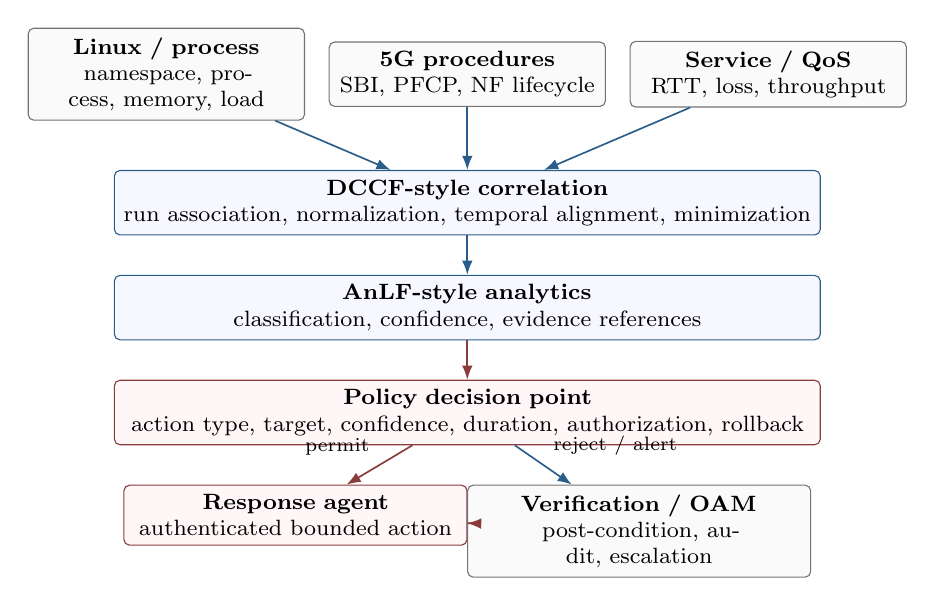
\begin{tikzpicture}[node distance=5mm and 3mm]
  \node[data,text width=.27\columnwidth] (linux) {\textbf{Linux / process}\\namespace, process, memory, load};
  \node[data,right=of linux,text width=.27\columnwidth] (fiveg) {\textbf{5G procedures}\\SBI, PFCP, NF lifecycle};
  \node[data,right=of fiveg,text width=.27\columnwidth] (svc) {\textbf{Service / QoS}\\RTT, loss, throughput};
  \node[box,below=8mm of fiveg,text width=.72\columnwidth] (dccf) {\textbf{DCCF-style correlation}\\run association, normalization, temporal alignment, minimization};
  \node[box,below=of dccf,text width=.72\columnwidth] (anlf) {\textbf{AnLF-style analytics}\\classification, confidence, evidence references};
  \node[secbox,below=of anlf,text width=.72\columnwidth] (pdp) {\textbf{Policy decision point}\\action type, target, confidence, duration, authorization, rollback};
  \node[secbox,below=of pdp,text width=.34\columnwidth,xshift=-.18\columnwidth] (agent) {\textbf{Response agent}\\authenticated bounded action};
  \node[data,below=of pdp,text width=.34\columnwidth,xshift=.18\columnwidth] (audit) {\textbf{Verification / OAM}\\post-condition, audit, escalation};
  \draw[arrow] (linux) -- (dccf);
  \draw[arrow] (fiveg) -- (dccf);
  \draw[arrow] (svc) -- (dccf);
  \draw[arrow] (dccf) -- (anlf);
  \draw[secarrow] (anlf) -- (pdp);
  \draw[secarrow] (pdp) -- node[above left,font=\scriptsize]{permit} (agent);
  \draw[arrow] (pdp) -- node[above right,font=\scriptsize]{reject / alert} (audit);
  \draw[secarrow] (agent) -- (audit);
\end{tikzpicture}
\caption{SecureNWDAF separates evidence correlation, analytics, policy authorization, bounded execution, and verification. Telemetry modalities are campaign-dependent and are never assumed to be simultaneously available.}
\Description{Three telemetry sources feed DCCF-style correlation, then AnLF-style analytics and a policy decision point. Approved actions reach an authenticated response agent and verification; rejected requests go to audit and escalation.}
\label{fig:architecture}
\end{figure}

Figure~\ref{fig:architecture} shows the core control and evidence paths. DCCF-style correlation is the first trust-preserving boundary: records are normalized and attached to one run before features are constructed. This prevents isolated events from unrelated experiments from becoming training samples that appear independent.

The analytics component consumes a feature representation that may contain Linux/process, virtual-network, protocol, and service-level dimensions. The precise set depends on the campaign. The paper therefore treats the feature vector as a typed interface rather than as a promise that every collector is active. A feature record stores both its value and its provenance source; missing modalities remain explicit.

The resulting diagnosis carries a confidence value and evidence references. It can recommend that an action be considered, but it cannot authorize an action. The PDP evaluates the diagnosis against the current policy context. This context can include the authorized NF target, action type, confidence threshold, maximum duration, operator authorization, and existence of a rollback transition.

After policy approval, SecIR converts the action into a typed workflow containing preconditions, execution parameters, post-conditions, and rollback. The authenticated response agent accepts only a narrow operation vocabulary. Verification observes the target state after execution and records whether the expected transition occurred. Failure can trigger rollback or escalation rather than silent continuation.

\subsection{Analytics path and evidence path}
The design maintains two related but distinct paths:
\begin{align}
\text{Evidence path: } & E \rightarrow \text{DCCF} \rightarrow X \rightarrow \text{AnLF},\\
\text{Control path: } & D \rightarrow \text{PDP} \rightarrow \text{SecIR} \rightarrow A \rightarrow V.
\end{align}
The first path concerns analytical correctness. The second concerns authorization and state transition correctness. This separation makes it possible to report a detector false positive without automatically counting it as a system-level security failure: policy may reject the response. Conversely, a correct diagnosis can still be followed by an execution failure, which belongs to the actuation layer rather than the classifier.

\subsection{Model lifecycle and evidence persistence}
Approved model artifacts are versioned independently from the operational policy. Each artifact is associated with training-split identifiers, feature schema, preprocessing configuration, software version, and evaluation manifest. The evidence store retains run identifiers, detector outputs, policy decisions, response requests, execution results, verification outcomes, and rollback state. This provenance is important for both auditability and debugging: a result can be re-evaluated against the exact data partition that produced it.

\section{Implementation on the free5GC Testbed}
\subsection{Two-machine deployment}
The prototype follows a deliberate two-machine split. The Ubuntu host runs the actual free5GC core, RAN/UE simulator, PDU-session traffic, collectors, controlled stimuli, and service probes. A separate GPU server hosts feature processing, model execution, the NWDAF-like analytics APIs, evidence storage, policy logic, and report generation. This separation reflects the practical research setup rather than pretending that the GPU machine is itself part of the free5GC core.

The free5GC environment follows the project's documented standalone architecture and can be paired with a simulated RAN/UE for reproducible user-plane and control-plane experiments~\cite{free5gcdocs,free5gcueransim}. The telemetry pipeline is intentionally read-oriented. Live observations can be transferred through an authenticated channel, while frozen campaigns are packaged as immutable archives. The analytics server does not need to install free5GC to reproduce offline model evaluation.

\begin{figure}[t]
\centering
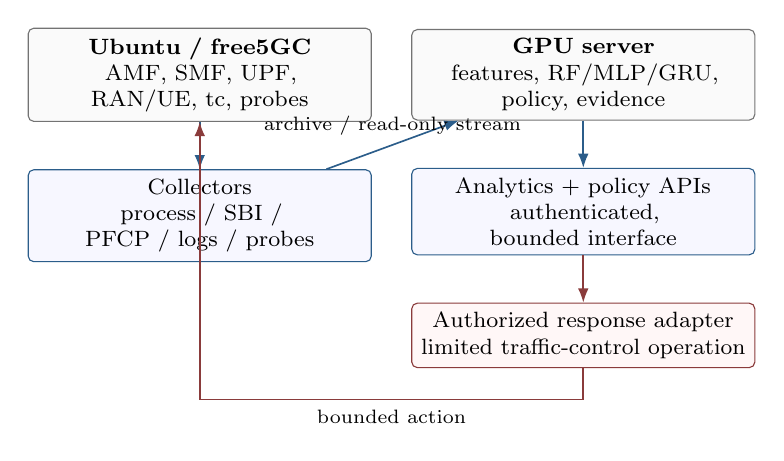
\begin{tikzpicture}[node distance=6mm and 5mm]
  \node[data,text width=.34\columnwidth] (core) {\textbf{Ubuntu / free5GC}\\AMF, SMF, UPF, RAN/UE, tc, probes};
  \node[data,right=of core,text width=.34\columnwidth] (gpu) {\textbf{GPU server}\\features, RF/MLP/GRU, policy, evidence};
  \node[box,below=of core,text width=.34\columnwidth] (collect) {Collectors\\process / SBI / PFCP / logs / probes};
  \node[box,below=of gpu,text width=.34\columnwidth] (api) {Analytics + policy APIs\\authenticated, bounded interface};
  \node[secbox,below=of api,text width=.34\columnwidth] (resp) {Authorized response adapter\\limited traffic-control operation};
  \draw[arrow] (core) -- (collect);
  \draw[arrow] (collect) -- node[above,font=\scriptsize]{archive / read-only stream} (gpu);
  \draw[arrow] (gpu) -- (api);
  \draw[secarrow] (api) -- (resp);
  \draw[secarrow] (resp.south) -- ++(0,-4mm) -| node[pos=.25,below,font=\scriptsize]{bounded action} (core.south);
\end{tikzpicture}
\caption{Two-machine implementation split. The free5GC host remains the authoritative network environment; the separate analytics server consumes archived or authenticated read-only observations and can request only policy-approved bounded actions.}
\Description{An Ubuntu free5GC host sends collector data to a separate GPU server. Analytics and policy APIs feed an authorized response adapter that performs a bounded action back on the testbed.}
\label{fig:testbed}
\end{figure}

\subsection{Collectors and data schema}
The collector schema uses explicit source types such as Linux/process telemetry, free5GC events, SBI events, PFCP records, and service probes. Each observation carries a run identifier and timestamp. Process records may include executable identity, process ancestry, resource state, and namespace-related fields when available. SBI and PFCP records are represented as parsed events rather than as raw payload dumps. Service-level signals include RTT, packet loss, throughput, and session state.

For each run, the pipeline records the available source modalities in metadata. A missing collector is represented by a missing modality rather than by a synthetic zero-valued stream. This matters for ablation: a model that performs well when protocol telemetry is unavailable is materially different from a model that silently benefits from an accidentally completed collector.

\subsection{Feature construction}
Let $W_{r,t}$ denote the observation window for run $r$ ending at time $t$. The feature vector is
\begin{equation}
\mathbf{x}_{r,t}=\phi(W_{r,t},c_{r,t})=
[\mathbf{x}^{\mathrm{host}}_{r,t},\mathbf{x}^{\mathrm{vnet}}_{r,t},
\mathbf{x}^{\mathrm{5g}}_{r,t},\mathbf{x}^{\mathrm{svc}}_{r,t},c_{r,t}],
\end{equation}
where $c_{r,t}$ includes authorized context such as NF identity, lifecycle phase, load profile, and scenario metadata. The classifier consumes aggregated window features for run-level scoring. Event-level rows are never treated as independent samples.

Feature families are chosen to capture complementary evidence. Host features represent process counts, distinct executables, resource pressure, namespace activity, and selected parent-child relations. Network features represent route or interface state when available. 5G features capture procedure outcomes, request counts, selected protocol transitions, and session events. Service features characterize the resulting network effect. The feature pipeline retains references to source records so that an anomalous feature can be inspected rather than interpreted as an opaque scalar.

\subsection{Policy and response implementation}
The policy layer represents each permitted operation as a structured object. The current response vocabulary is intentionally limited to operator alerting and a temporary traffic-control transition. An action contains an action identifier, target, expiration time, authorization record, and rollback information. The response agent authenticates incoming requests, checks replay protection, and dispatches only recognized operation types.

For the implemented traffic-control action, the state transition is conceptually
\begin{equation}
\texttt{fq\_codel} \rightarrow \texttt{tbf}(R) \rightarrow \texttt{fq\_codel},
\end{equation}
where $R$ is a configured rate bound. The particular rate is treated as an experimental parameter and must be reported with the new campaign configuration. Verification checks that the target interface reaches the intended queue discipline, that the action is applied only to the authorized target, and that the rollback operation restores the recorded original state.

\section{Threat Model and Scenario Taxonomy}
\subsection{Adversary assumptions}
The attacker is assumed to control or influence a lower-trust component such as a compromised workload, exposed management interface, dependency, or API-facing process. The attacker may attempt to cross an isolation boundary, exhaust host resources, manipulate virtual-network state, or generate abnormal control/user-plane behavior. The attacker does not initially control the trusted policy engine or authenticated response agent.

This threat model deliberately does not require a public CVE or a portable exploit. Controlled laboratory stimuli are preferable for this study because they allow repeated runs, known ground truth, and measured service effects. The objective is to test whether the telemetry and control architecture can distinguish behavior and react safely, not to demonstrate exploit development.

\subsection{Scenario families}
The new experiment uses only attack families for which the current testbed already has a safe and repeatable stimulus mechanism. The exact implemented IDs are discovered from the repository before the campaign is launched. Scenarios without a safe mechanism remain excluded rather than being simulated with fabricated traces.

\begin{table}[t]
\caption{Experimental scenario taxonomy and intended evidence.}
\label{tab:taxonomy}
\centering\scriptsize
\setlength{\tabcolsep}{2.7pt}
\renewcommand{\arraystretch}{1.07}
\begin{tabularx}{\columnwidth}{>{\raggedright\arraybackslash}p{0.22\columnwidth} >{\raggedright\arraybackslash}p{0.31\columnwidth} X}
\toprule
Family & Controlled stimulus & Representative evidence \\
\midrule
Normal & benign startup, session, and sustained traffic & lifecycle, process, service KPIs \\
Namespace / privilege & controlled namespace or capability transition & ancestry, namespace, capability state \\
Runtime boundary & controlled runtime-interface access & socket, process lineage, identity \\
Virtual network & controlled bridge / route / port state change where supported & interface, flow, forwarding state \\
Resource pressure & bounded CPU/memory/process/network pressure & resources, NF health, RTT, loss \\
SBI / HTTP2 & abnormal request burst or sequence & request rate, errors, procedure state \\
PFCP & controlled abnormal session-management behavior & PFCP events, session outcomes \\
Composite & two-stage stimulus with independent benign load & cross-layer temporal correlation \\
\bottomrule
\end{tabularx}
\end{table}

The taxonomy is deliberately behavioral. It avoids assigning maliciousness to one primitive event. For example, a namespace operation may be normal during legitimate process initialization. A malicious or anomalous interpretation requires contextual evidence such as unexpected ancestry, target namespace, capability state, or subsequent service impact.

\subsection{Trust boundaries and failure containment}
There are four security boundaries. First, collectors are read-oriented evidence producers. Second, the analytics service is computationally privileged but not operationally authorized. Third, the PDP is the authorization boundary for state-changing operations. Fourth, the response agent is a narrow execution endpoint whose accepted verbs are smaller than the action space available to the underlying Linux host.

This decomposition is a direct mitigation for a common failure mode of AI-driven automation: the detector is allowed to issue the same interface used by administrators. SecureNWDAF instead requires a policy-valid transition. A false positive can therefore be blocked by a target or confidence constraint; a correct diagnosis can still be blocked if the action is not authorized; and an execution failure can be observed independently of the detector.

\section{New Experimental Methodology}
\subsection{Campaign design}
The earlier pilot and supplemental result sets are explicitly discarded for the new study. No previous metric, model checkpoint, confusion matrix, latency result, or response count is reused as a result in this paper. The new campaign begins from a clean experiment namespace with a fresh campaign identifier and regenerated run manifests.

The campaign is organized into five evaluation studies:
\begin{enumerate}[leftmargin=*]
\item \textbf{E1 Detection.} Evaluate B0 (load-threshold), B1 (Random Forest), and optional neural backends on the same leakage-safe run-level split.
\item \textbf{E2 Modality ablation.} Compare host-only, 5G-only, service-only, and combined feature sets on campaigns where the corresponding evidence is genuinely available.
\item \textbf{E3 Generalization.} Hold out stimulus seeds and at least one operating-load condition from model development, then evaluate the fixed model without retuning.
\item \textbf{E4 Online behavior.} Measure end-to-end detection latency and inference processing time on live traffic with the detector operating against the real free5GC path.
\item \textbf{E5 Response safety.} Execute paired alert-only and policy-bounded response trials and measure policy correctness, enforcement delay, service impact, and restoration success.
\end{enumerate}

The exact repetition count is a campaign configuration rather than a hidden assumption. The recommended minimum is five independent repetitions per scenario/load/seed cell, with more repetitions for the primary test cells when the testbed remains stable. The experiment controller must report the resulting counts before analysis and stop the campaign if runs overlap or share an output directory.

\begin{table*}[t]
\caption{New evaluation matrix. Exact counts are instantiated from the campaign configuration and recorded in the manifest.}
\label{tab:experiments}
\centering\scriptsize
\setlength{\tabcolsep}{3.1pt}
\renewcommand{\arraystretch}{1.08}
\begin{tabularx}{\textwidth}{>{\raggedright\arraybackslash}p{0.08\textwidth} >{\raggedright\arraybackslash}p{0.18\textwidth} >{\raggedright\arraybackslash}p{0.20\textwidth} >{\raggedright\arraybackslash}X >{\raggedright\arraybackslash}p{0.14\textwidth}}
\toprule
Study & Question & Controlled variables & Required measurements & Split / analysis rule \\
\midrule
E1 & RQ1 & scenario, background load, repetition, stimulus seed & precision, recall, F1, FPR, confusion matrix, inference time & run-level train/val/test \\
E2 & RQ2 & telemetry modality availability & macro F1, per-class recall, false positives, feature cost & same runs where possible \\
E3 & RQ2 & unseen seed and unseen load & fixed-model F1, per-class recall, calibration & no retuning on test cells \\
E4 & RQ3 & live load, attack timing, detector mode & detection latency, inference latency, packet loss, RTT & repeated online trials \\
E5 & RQ3 & alert-only vs response, bounded rate limit & policy decision time, enforcement time, restoration, service KPIs & paired trials \\
Overhead & RQ1/RQ3 & collector mode, load, telemetry frequency & CPU, memory, telemetry bytes, process overhead & matched baseline \\
\bottomrule
\end{tabularx}
\end{table*}

\subsection{Data partitioning and leakage prevention}
The split is defined at the run level. Suppose $R$ is the set of all completed runs. We construct disjoint sets
\begin{equation}
R=R_{\mathrm{train}}\cup R_{\mathrm{val}}\cup R_{\mathrm{test}},
\qquad
R_i\cap R_j=\emptyset \; (i\\eq j).
\end{equation}
All windows derived from the same run remain in one partition. No model hyperparameter is selected using the held-out test set. Standardization, feature selection, and threshold calibration are learned only from the training/validation data.

For E3, the partition additionally holds out stimulus seeds. Let $s$ denote a stimulus seed. The test set contains seeds absent from the model-development set. Where feasible, one load profile is also held out. This design is stricter than random event-row splitting because it asks whether a detector recognizes the behavioral family when the exact event timing or operating condition changes.

\subsection{Baselines and ablations}
B0 is a conventional threshold detector based on load or resource pressure. Its threshold is selected using the validation partition only. B1 is a Random Forest using the full run-level feature vector. Optional GPU backends, such as an MLP or temporal GRU, use the same train/validation/test partitions and receive no privileged information.

Modality ablations test whether cross-layer context adds information. Host-only features represent the minimum Linux-centric detector. 5G-only features use real parsed SBI/PFCP or procedure observations when present. Service-only features capture the observable effect on user-plane performance. The combined model receives all modalities available in that campaign. An ablation is invalid if the supposedly removed modality leaks through a derived feature or if the missing modality is replaced with a fabricated constant stream.

\subsection{Metrics}
Detection quality is reported using precision, recall, F1, macro F1, and false-positive rate. For a binary detector,
\begin{equation}
\mathrm{Precision}=\frac{TP}{TP+FP},\quad
\mathrm{Recall}=\frac{TP}{TP+FN},\quad
F_1=\frac{2PR}{P+R}.
\end{equation}
False-positive rate is reported as $FP/(FP+TN)$ on the defined normal population. For multiclass analysis, macro F1 is the unweighted mean of classwise F1 values.

Latency is reported using timestamps collected at the experiment controller rather than host logs whose clocks may drift. We separate (i) stimulus-to-analytics latency, (ii) analytics-to-policy latency, (iii) policy-to-enforcement latency, and (iv) enforcement-to-verified-restoration time. For live traffic, service impact is reported through RTT, packet loss, throughput, and session status. Overhead is reported as CPU utilization, memory usage, and telemetry bytes per second under matched load conditions.

\subsection{Statistical reporting}
Because controlled runs are grouped observations, uncertainty must be reported at the run level. The primary result should include a confidence interval obtained by resampling complete runs rather than individual event rows. Bootstrap intervals can be computed over the held-out runs for F1 and latency. For paired response trials, the same trial seed should be used for the alert-only and response conditions when safe, allowing paired differences in service metrics and restoration time.

The report must also include the number of valid and invalid runs, dropped records, collector availability, and missing telemetry by source type. Failed runs are never silently omitted. A run is excluded only with a recorded reason and a corresponding entry in the campaign manifest.

\section{Evaluation and Results Reporting}
\subsection{Reproducible result contract}
This section is intentionally written as the final report structure for the new campaign. All values marked \TBD{} must be replaced from machine-generated manifests after the new experiments complete. No values from earlier pilot or supplemental campaigns are valid inputs to this section.

\begin{table}[t]
\caption{Primary results table to be populated from the new campaign.}
\label{tab:primary}
\centering\scriptsize
\setlength{\tabcolsep}{3pt}
\renewcommand{\arraystretch}{1.08}
\begin{tabular}{lll}
\toprule
Measure & Detector & New-campaign result \\
\midrule
F1 & B0 & \BZeroFone \\
F1 & B1 Random Forest & \RFFOne \\
Precision & B1 Random Forest & \RFPrecision \\
Recall & B1 Random Forest & \RFRecall \\
FPR & B1 Random Forest & \RFFPR \\
F1 & CUDA MLP & \MLPFOne \\
F1 & Temporal GRU & \GRUFOne \\
\bottomrule
\end{tabular}
\end{table}

The first evaluation question is whether the richer run-level feature set improves controlled anomaly discrimination over the threshold baseline. The comparison must be made on exactly the same held-out runs. The result should report the confusion matrix, per-class recall, and the distribution of prediction confidence. A single F1 number is insufficient because the application is security-sensitive and the operational consequence of false positives and false negatives is asymmetric.

The second question is whether cross-layer evidence improves robustness beyond the conditions represented during model development. Results from E2 should therefore show both overall performance and per-modality performance. A combined model that improves average F1 but becomes highly sensitive to one telemetry source would have a different operational profile from a model whose decision remains stable when a source is temporarily unavailable.

\subsection{Unseen-stimulus and unseen-load evaluation}
E3 is the principal generalization test. After the development split is frozen, the model is evaluated on new stimulus seeds and, where feasible, a held-out load profile. The paper should report both aggregate metrics and class-specific behavior. A drop in performance is not hidden; instead, the magnitude of the drop is interpreted as evidence about deployment sensitivity.

The analysis should also test whether the model is learning attack identity or merely workload intensity. A strong sign of load confounding is a large performance decrease when the same behavioral family is generated under a different background load. Conversely, stable recall across held-out loads provides evidence that the detector uses more than one scalar resource signal.

\subsection{Online latency and service impact}
The online experiment reports a latency decomposition rather than a single number. Let $T_0$ be the timestamp of the first attack-defining event, $T_1$ the time the analytics result is generated, $T_2$ the time the PDP returns a decision, and $T_3$ the time the bounded action is verified. Then
\begin{align}
L_{\mathrm{detect}} &= T_1-T_0,\\
L_{\mathrm{policy}} &= T_2-T_1,\\
L_{\mathrm{enforce}} &= T_3-T_2.
\end{align}
The paper should report medians and tail values where the number of trials permits. Service impact should be compared against an alert-only or no-response condition rather than assuming that a successful command implies service recovery.

\begin{table}[t]
\caption{Online and response measurements to populate.}
\label{tab:online}
\centering\scriptsize
\setlength{\tabcolsep}{3pt}
\renewcommand{\arraystretch}{1.08}
\begin{tabular}{lll}
\toprule
Measure & Condition & Result \\
\midrule
Detection latency & Live B1 & \DetLat \\
Policy/enforcement latency & B2 & \RespLat \\
Apply success & B2 rate limit & \ApplyRate \\
Restore success & B2 rollback & \RestoreRate \\
False action & Benign trials & \FalseAction \\
CPU overhead & Collector + analytics & \CPUOverhead \\
Telemetry rate & Full collector set & \TelemetryOverhead \\
\bottomrule
\end{tabular}
\end{table}

\subsection{Response correctness}
Response correctness is treated as a conjunction of policy and state-transition properties. A trial is considered successful only if (i) authentication succeeds, (ii) replay protection permits exactly one request, (iii) the PDP accepts an allow-listed action, (iv) the agent applies the action to the intended target, (v) verification observes the expected state, and (vi) rollback restores the recorded original state when required.

The response experiment should also include negative authorization tests: wrong target, unsupported action type, expired request, insufficient confidence, duplicate request identifier, missing rollback specification, and unauthorized caller. These cases should be rejected before a state-changing operation reaches the host. The rejection count should therefore be reported separately from detector performance.

\subsection{Expected result interpretation}
The final paper should avoid collapsing E1--E5 into one ``system accuracy'' number. Detection quality answers whether the analytics component distinguishes controlled behaviors. Ablations explain which evidence contributes. Generalization tests explain sensitivity to new conditions. Latency and service metrics characterize operational timing and impact. Response trials validate authorization and reversible state transitions. A system may therefore have a good detector but a poor response implementation, or a safe response boundary even when the detector is imperfect.

\section{Security Analysis and Engineering Discussion}
\subsection{Why policy must be separate from inference}
The core security argument of SecureNWDAF is that a model output is an input to authorization, not authorization itself. Suppose the model produces a high-confidence diagnosis. A safe system must still ask whether the target is authorized, whether the action is allowed for that target, whether the duration is within policy, and whether a verified rollback is available. These checks are deterministic policy predicates rather than learned behavior.

This separation creates a form of failure containment. A model error need not become a host-level change. A policy error can be audited independently of the model's confidence. An execution failure can be detected after the state transition and trigger rollback or escalation. The design is therefore compatible with a defense-in-depth interpretation of AI-enabled management rather than treating the model as a trusted administrator.

\subsection{Evidence provenance and auditability}
Cross-layer analytics can easily become difficult to audit if raw events, features, and decisions are mixed. SecureNWDAF keeps separate records for raw observations, feature derivation, model outputs, policy decisions, response execution, and verification. Each stage retains a reference to its input. This allows an investigator to reconstruct not only what the system did, but why it believed an action was warranted and which observations supported the decision.

The provenance model also reduces a common reproducibility error: reporting many event rows as though they were independent experiments. The unit of controlled variation is the run. Event rows are inputs to the run, not additional replications. This distinction is particularly important for 5G security datasets, where one abnormal sequence can generate thousands of closely correlated observations~\cite{5gprovgen}.

\subsection{Confidentiality and evidence minimization}
The prototype favors metadata, event counts, process identity, network state, and service KPIs over subscriber payloads and authentication secrets. The design does not require user-plane payload inspection. Nevertheless, cross-layer metadata can become sensitive when correlated. A production deployment would need explicit retention, role-based access control, encryption, and purpose limitation. The current research prototype should therefore be understood as an evidence-minimized laboratory design, not as a complete privacy compliance framework.

\subsection{Least privilege and response-agent risk}
Authentication and allow-listing do not eliminate all response risks. The execution environment can still have more operating-system privilege than is strictly required by the allowed action vocabulary. A secure deployment should minimize the response agent's Linux privileges, restrict accessible interfaces, and separate the agent from unrestricted shell execution. The policy boundary is thus necessary but not sufficient: it must be reinforced by operating-system least privilege and secure key management~\cite{nistcontainer,nistzero}.

\subsection{Operational trade-offs}
Cross-layer monitoring improves context but increases telemetry volume and processing cost. Fine-grained process or eBPF observations can provide useful precursors at the expense of CPU overhead and data transport. Protocol telemetry provides network semantics but may be intermittent depending on the experiment. Service-level probes reveal actual user-plane consequences but can lag behind the initiating event. The experimental methodology therefore evaluates both detection quality and overhead, allowing a deployment decision to be based on a measurable trade-off rather than an assumption that more telemetry is always better.

\section{Security Properties and Failure Cases}
\subsection{Policy safety properties}
The response layer can be stated as a set of invariants that are independent of the classifier. Let $A_{\mathrm{exec}}$ denote an action observed at the response adapter and let $A_{\mathrm{permit}}$ denote the set of actions accepted by the PDP. The first invariant is authorization closure:
\begin{equation}
A_{\mathrm{exec}} \subseteq A_{\mathrm{permit}}.
\end{equation}
An action that is not present in the PDP decision cannot reach the state-changing adapter. The second invariant is target closure: an approved action is bound to the target encoded in the policy decision and cannot be redirected by the model output or by a later API field. The third invariant is temporal closure: every bounded action has an explicit expiration or rollback condition.

The fourth invariant is provenance closure. Each operational transition must have a corresponding diagnosis, policy decision, request identifier, and verification record. This does not prove that the diagnosis itself was correct; it ensures that the execution path can be reconstructed after the fact. The fifth invariant is failure visibility: authentication failure, policy rejection, adapter failure, and verification failure are recorded as distinct events. These invariants allow response safety to be evaluated without assuming a perfect anomaly detector.

\begin{table}[t]
\caption{Policy predicates and observable failure cases.}
\label{tab:policy}
\centering\scriptsize
\setlength{\tabcolsep}{2.5pt}
\renewcommand{\arraystretch}{1.08}
\begin{tabularx}{\columnwidth}{>{\raggedright\arraybackslash}p{0.22\columnwidth} X X}
\toprule
Predicate & Allowed condition & Failure response \\
\midrule
Authentication & trusted caller/key & reject and audit \\
Replay & unused request identifier & reject duplicate \\
Action type & allow-listed verb & reject without host change \\
Target & authorized NF/interface & reject wrong scope \\
Confidence & $p\ge\tau_p$ & observe / escalate \\
Duration & within policy bound & reject or clip to bound \\
Rollback & verified inverse transition exists & reject unsafe action \\
Verification & expected post-condition observed & rollback / escalate \\
\bottomrule
\end{tabularx}
\end{table}

These properties are intentionally simple because deterministic controls are easier to audit than a learned safety policy. They also make the implementation extensible: a future action can be added only after its type, target, duration, authorization, and rollback semantics are defined.

\subsection{Failure-case walkthrough}
Consider four representative failure cases. First, if the detector produces a high-confidence diagnosis but the target is outside the policy scope, the PDP rejects the action. Second, if an authorized response request is retransmitted, replay protection accepts at most the first valid request. Third, if the adapter changes the state but verification cannot observe the expected post-condition, the workflow marks the response as failed and invokes the configured recovery path. Fourth, if the analyzer itself becomes unavailable, the monitoring system can continue to ingest evidence and generate an operator alert without granting the analyzer a bypass path to execution.

The intended fail-closed behavior applies specifically to state-changing actions. Read-only telemetry collection and evidence persistence may continue during a policy-service outage, but no response action should be inferred from an unavailable policy decision. This distinction is important because an analytics component can be degraded without forcing the network into an uncontrolled operational state.

\subsection{Why the testbed matters}
The policy properties would be difficult to validate on an abstract dataset alone because the final invariant concerns an actual state transition. free5GC supplies a concrete 5G Core environment in which network functions, SBI interactions, PFCP state, user-plane paths, and Linux traffic-control state can be observed together~\cite{free5gc,free5gcdocs}. The two-machine arrangement further separates the place where the network state exists from the place where models and policy logic execute. This permits experiments to distinguish analytics failure from execution failure.

\section{Experimental Orchestration and Reproducibility Protocol}
\subsection{Run state machine}
Each experiment run follows a state machine:
\begin{equation*}
\begin{aligned}
&\texttt{ALLOCATE}\rightarrow\texttt{BASELINE}\rightarrow\texttt{STIMULATE}\\[-1mm]
&\qquad\rightarrow\texttt{CAPTURE}\rightarrow\texttt{VERIFY}\rightarrow\texttt{CLOSE}.
\end{aligned}
\end{equation*}
The controller allocates a fresh run directory and identifier before any process starts. The baseline state records interface configuration, process inventory, active sessions, and service probes. Only after the baseline is stable is the controlled stimulus started. Capture ends at a deterministic time or after a defined post-stimulus interval. Verification checks file completeness, timestamp monotonicity, required metadata, and expected run closure.

A run is invalid if the controller detects overlapping writers, missing mandatory metadata, clock anomalies that prevent ordering, or an incomplete archive. Invalid runs remain visible in the manifest and are not silently converted into negatives. This is important for security experiments because a failed collector can otherwise look like a benign sample and bias the classifier.

\subsection{Campaign manifest}
The campaign manifest is the authoritative experiment ledger. For every run it stores the scenario family, exact scenario identifier, seed, background-load profile, collector availability, software version identifiers, start and end times, validity state, and partition assignment. The campaign-level manifest additionally records the feature schema hash, model configuration, policy configuration, and response vocabulary.

The following information is required before a new campaign is considered frozen:
\begin{enumerate}[leftmargin=*]
\item the complete set of valid and invalid run identifiers;
\item the run-level train/validation/test partition;
\item the mapping from scenario and seed to each run;
\item collector availability and dropped-record counts;
\item the exact model and preprocessing configuration; and
\item the response-policy configuration and action audit records.
\end{enumerate}
This structure ensures that an evaluator can distinguish a change in model code from a change in data generation.

\subsection{Recommended new-campaign scale}
The paper does not hard-code one exact repetition count because the safe limit depends on testbed stability. A practical target is at least five valid repetitions for each scenario/load/seed cell, with additional repetitions allocated to the main test cells. If the repository can reliably sustain ten repetitions per cell without overlapping processes, that larger count should be preferred for the primary analysis. The important property is that the count is predetermined in configuration and that the final paper reports the exact completed count rather than stopping opportunistically when a desired metric is reached.

For the unseen-stimulus experiment, the seed set is partitioned before model training. For example, seeds $s_1\ldots s_m$ can be divided into development and held-out groups, with the held-out seeds generated only after the model configuration is frozen. The same principle applies to load profiles. This makes the test a genuine generalization measurement rather than another round of parameter tuning.

\subsection{Analysis pipeline}
The frozen analysis should be executable with one command from the campaign manifest. The analysis script loads the exact partition, derives features using the stored schema, evaluates B0/B1 and optional neural backends, computes confidence intervals over complete runs, generates confusion matrices and per-class tables, and writes a machine-readable summary. A separate report generator converts that summary into the tables used in this paper.

This design reduces the chance of transcription errors and makes the paper itself an auditable view of the experiment. It also helps preserve the distinction between exploratory plots and primary metrics: exploratory analysis may use validation data, while the primary test results are generated only once from the frozen test partition.

\section{Reproducibility and Artifact Plan}
The experiment is designed so that a fresh campaign can be reconstructed from the testbed configuration, scenario manifest, collector configuration, run manifests, and model configuration. Each run receives a globally unique identifier. A campaign directory contains an immutable manifest describing the software versions, host configuration, background-load profile, scenario seed, telemetry sources, start/stop timestamps, and validity status.

The experiment controller must enforce one output directory per run. This prevents overlapping processes from writing to the same archive and avoids the class of race that can silently corrupt a dataset while leaving superficially valid files behind. Campaign generation is therefore serialized or uses isolated directories with an explicit run lock.

For the frozen analytical evaluation, the following artifacts are required: raw run archives, the complete-run split manifest, the feature schema, the trained model artifact, preprocessing parameters, inference outputs, evaluation scripts, and a machine-readable result summary. The paper's primary tables should be generated from that result summary rather than hand-entered. A cryptographic hash of the final campaign archive should be recorded after the campaign is frozen.

The repository reference is included only as the implementation source, not as a substitute for experimental detail. The paper remains self-contained: the testbed topology, measurement definitions, split rules, response constraints, and result-generation process are described here. This is particularly important for a forum paper centered on an open-source platform, where other researchers should be able to recreate the evaluation without assuming undocumented state in the author's environment.

\section{Deployment Considerations and Generalization}
\subsection{From laboratory prototype to operational service}
The present implementation is intentionally narrower than a production security platform. It nevertheless exposes several interfaces that matter for a future deployment. First, telemetry ingestion must be versioned because a feature produced by one free5GC or Linux configuration may not have identical semantics on another host. Second, model artifacts need an explicit identity and compatibility record. A policy decision should reference the artifact version used to produce the diagnosis so that an operator can reconstruct the analytical context later.

Third, the response interface should be treated as a security-sensitive management service rather than as an ordinary utility API. Authentication keys must be rotated, request identifiers must be unique, and the agent should expose only the minimum command surface needed by the current action vocabulary. The laboratory implementation uses a small allow-list because this makes the security argument testable. A future deployment could use a capability-based interface or a dedicated privileged helper rather than a general-purpose sudo context.

Fourth, response policy should be separated from model training. Model changes affect what the analyzer believes; policy changes affect what the network is permitted to do. Combining both into one version number would make incident reconstruction difficult and could cause a model update to implicitly change operational authority. SecureNWDAF instead treats policy and model artifacts as independently auditable inputs to the decision.

\subsection{Integration with free5GC operational state}
The free5GC platform exposes multiple control and user-plane relationships that can be useful for security context. The SBI provides NF-to-NF service interactions, while PFCP connects the control and user planes for session state and forwarding behavior. User-plane measurements provide the external consequence of those internal states. A cross-layer analyzer can therefore distinguish a protocol event that has no observable service effect from one followed by a change in session behavior.

The implementation does not require invasive modification of free5GC for every telemetry source. Read-only logs, protocol event streams, host observation, and active service probes can be collected independently and correlated through a run identifier. This approach lowers coupling between the analytics research code and the core-network implementation, which is useful when the underlying free5GC release changes.

\begin{table}[t]
\caption{Implementation interfaces and security assumptions.}
\label{tab:interfaces}
\centering\scriptsize
\setlength{\tabcolsep}{2.5pt}
\renewcommand{\arraystretch}{1.08}
\begin{tabularx}{\columnwidth}{>{\raggedright\arraybackslash}p{0.22\columnwidth} X X}
\toprule
Interface & Research purpose & Primary assumption \\
\midrule
Telemetry stream & read-only host/5G/service evidence & source identity and timestamp are trustworthy enough for correlation \\
Analytics API & submit feature windows / obtain diagnosis & authentication and schema validation \\
Policy API & evaluate proposed action & fail closed for state-changing requests \\
Response API & execute allow-listed operation & minimal privilege and target binding \\
Audit store & preserve decision provenance & append-oriented integrity and controlled access \\
Rollback path & restore prior state & inverse operation remains valid and verifiable \\
\bottomrule
\end{tabularx}
\end{table}

\subsection{Generalization beyond one model}
Although the primary detector is a Random Forest, the architecture is model-agnostic at the policy boundary. A future detector may output a calibrated probability, a ranked set of hypotheses, or a temporal anomaly score. The policy engine can consume a normalized diagnosis object as long as the object identifies the model artifact, confidence semantics, target scope, and evidence references. This decoupling allows ML research to evolve without requiring the response agent to understand the internals of every model.

The same principle applies to deployment location. The analyzer may run on the separate GPU server, on a network-management host, or at an edge gateway. The safety boundary remains the same: evidence is correlated, a diagnosis is produced, policy authorizes a bounded operation, and verification closes the loop. The placement can therefore be optimized later for latency and telemetry cost without redesigning the operational trust model.

\section{Limitations and Extension Toward 6G NTN}
\subsection{Current limitations}
The current work is a controlled laboratory evaluation on a terrestrial open-source 5G Core. Its main validity boundaries are therefore clear. First, the attack space is limited to repeatable laboratory stimuli rather than the full space of real-world compromises. Second, not every telemetry collector is active in every campaign, so cross-layer claims must be interpreted according to the actual modality matrix. Third, the detector is evaluated primarily with run-level features rather than a full causal model of service recovery. Fourth, the response action is intentionally narrow. Fifth, a two-machine topology cannot establish carrier-scale scalability.

The new study also does not attempt to prove that any model architecture is universally superior. The Random Forest is a reference detector chosen for transparent handling of heterogeneous tabular features. GPU-side models are useful for exploring whether richer temporal or nonlinear representations help, but the core contribution is the experimental and control architecture rather than an algorithmic claim about neural networks.

\subsection{6G non-terrestrial networks}
Future 6G systems increasingly consider integrated terrestrial and non-terrestrial networking. Research on NTN highlights the need to accommodate propagation-delay constraints, mobility, dynamic coverage, gateway relationships, and the integration of terrestrial and satellite segments~\cite{ntn5gspace,ntnrel17,ntn6g,role6gntn}. These properties do not require a fundamentally different analytics control loop, but they add new context dimensions.

For a future NTN-aware version, the feature representation can be extended as
\begin{equation}
\mathbf{x}^{6G}_t=
[\mathbf{x}^{\mathrm{Linux}}_t,\mathbf{x}^{\mathrm{5G}}_t,
\mathbf{x}^{\mathrm{NTN}}_t,\mathbf{x}^{\mathrm{SLO}}_t,c_t],
\end{equation}
where $\mathbf{x}^{\mathrm{NTN}}_t$ may include satellite or platform identity, beam state, gateway association, propagation delay, feeder-link condition, and mobility/handover information. The DCCF abstraction can then correlate terrestrial core observations with future NTN producers.

An integrated TN--NTN deployment may also introduce additional aggregation and signaling requirements across segments~\cite{multintn}. This makes the policy boundary more important rather than less: a condition observed in a satellite or gateway segment should not automatically authorize a core-network state change. A future SecureNWDAF extension could instead require domain-specific authorization and rollback rules for each target class.

Distributed analytics placement is another research opportunity. A centralized analyzer offers global visibility but may require transporting large telemetry volumes. Edge or gateway analytics can reduce transport cost and reaction time but has a smaller global context. 6G architecture work increasingly considers distributed AI and computing as first-class components~\cite{perspectives6g}. SecureNWDAF can provide a policy abstraction above either placement model, provided that model identity, domain authority, evidence provenance, and rollback semantics remain explicit.

The NTN discussion is intentionally an extension proposal rather than an evaluated capability. NTN experiments should first establish realistic telemetry producers and mobility/load traces before any satellite- or gateway-level response is considered.

\section{Conclusion}
This paper presents SecureNWDAF, a free5GC-based security analytics architecture that treats cross-layer evidence and safe actuation as separate research problems. The design uses NWDAF terminology to align analytics responsibilities with 3GPP concepts, while keeping the implementation explicitly external to the standardized NWDAF function. DCCF-style correlation preserves run-level provenance; an AnLF-style analyzer produces an evidence-backed diagnosis; policy evaluation remains outside the model; and a narrow authenticated response agent performs only authorized and reversible operations.

The new experimental methodology is designed to provide stronger evidence than a single held-out pilot score. It evaluates leakage-safe run-level detection, telemetry ablation, unseen stimulus seeds, unseen operating loads, online latency, response correctness, service impact, and system overhead. These studies produce separate measurements for analytical quality and control-path safety, avoiding the misleading practice of collapsing them into one system score.

All numerical values in this submission draft are intentionally withheld until the new campaign is executed. This prevents old pilot measurements from being carried forward and makes the final paper's claims directly traceable to one frozen experimental generation. Once the campaign is complete, the tables and result narrative should be populated automatically from the campaign manifest and then audited against the raw run archives.

The resulting framework is intended as a reproducible basis for research on secure, open, programmable 5G infrastructures. Its longer-term direction is toward richer cross-domain analytics and policy-bounded automation in 6G, including terrestrial/non-terrestrial integration, but such extensions should be evaluated only after their telemetry, authority, and rollback semantics can be measured rather than assumed.

\balance
\begin{thebibliography}{99}
\small

\bibitem{ts23288}
3GPP. \emph{Architecture enhancements for 5G System (5GS) to support network data analytics services}. TS 23.288, Release 20, version 20.2.0, 2026.

\bibitem{ts29520}
3GPP. \emph{5G System; Network Data Analytics Services; Stage 3}. TS 29.520, Release 20, version 20.1.0, 2026.

\bibitem{free5gc}
free5GC Project. \emph{free5GC: Open Source Core Network Implementation}. 2026. \url{https://free5gc.org/}.

\bibitem{free5gcdocs}
free5GC Project. \emph{free5GC Documentation and Design Guides}. 2026. \url{https://free5gc.org/doc/}.

\bibitem{free5gcueransim}
free5GC Project. \emph{free5GC and UERANSIM deployment tutorial}. 2026. \url{https://free5gc.org/guide/UERANSIM/UERANSIM/}.

\bibitem{nwdafcode}
H. Qin. \emph{NWDAF-like Security Analytics Prototype}. GitHub repository, 2026. \url{https://github.com/haochenq-moss/nwdaf-research}.

\bibitem{mlnwdaf}
A. Mekrache, K. Boutiba, and A. Ksentini. Combining Network Data Analytics Function and Machine Learning for Abnormal Traffic Detection in Beyond 5G. In \emph{IEEE GLOBECOM}, Kuala Lumpur, Malaysia, Dec. 2023. doi:10.1109/GLOBECOM54140.2023.10436766.

\bibitem{yuan2022}
Y. Yuan, C. Gehrmann, J. Sternby, and L. Barriga. Insight of Anomaly Detection with NWDAF in 5G. In \emph{2022 International Conference on Computer, Information and Telecommunication Systems (CITS)}, 2022, pp. 1--6. doi:10.1109/CITS55221.2022.9832914.

\bibitem{oliveira2024}
J. M. Oliveira, J. Almeida, E. de Britto e Silva, L. F. Rodrigues Moreira, R. Moreira, F. O. Silva, D. F. Macedo, and J. M. Nogueira. Anomaly Detection Employing a 5G Core Data Analytics Framework. In \emph{2024 IEEE 13th International Conference on Cloud Networking (CloudNet)}, 2024, pp. 1--9. doi:10.1109/CloudNet62863.2024.10815754.

\bibitem{ardestani2026}
F. S. Ardestani, N. Saha, N. Limam, and R. Boutaba. Towards NWDAF-enabled Analytics and Closed-Loop Automation in 5G Networks. In \emph{IEEE/IFIP Network Operations and Management Symposium (NOMS)}, Rome, Italy, May 2026.

\bibitem{akon2023}
M. Akon, T. Yang, Y. Dong, and S. R. Hussain. Formal Analysis of Access Control Mechanism of 5G Core Network. In \emph{Proceedings of the 2023 ACM SIGSAC Conference on Computer and Communications Security (CCS '23)}, 2023, pp. 666--680. doi:10.1145/3576915.3623113.

\bibitem{dolente2024}
F. Dolente, R. G. Garroppo, and M. Pagano. A Vulnerability Assessment of Open-Source Implementations of Fifth-Generation Core Network Functions. \emph{Future Internet}, 16(1), 2024. doi:10.3390/fi16010001.

\bibitem{5gcfuzz}
Y. Sun et al. 5GC-Fuzz: Finding Deep Stateful Vulnerabilities in 5G Core Network with Black-Box Fuzzing. In \emph{IEEE INFOCOM}, 2025.

\bibitem{corecrisis}
Y. Dong et al. CoreCrisis: Threat-Guided and Context-Aware Iterative Learning and Fuzzing of 5G Core Networks. In \emph{34th USENIX Security Symposium}, 2025.

\bibitem{5gprovgen}
A. Abouelkhair, K. Majdi, N. Limam, M. A. Salahuddin, and R. Boutaba. 5GProvGen: 5G Provenance Dataset Generation Framework. In \emph{2024 20th International Conference on Network and Service Management (CNSM)}, Prague, Czech Republic, 2024, pp. 1--9. doi:10.23919/CNSM62983.2024.10814296.

\bibitem{ebpf}
D. Soldani et al. eBPF: A New Approach to Cloud-Native Observability, Networking and Security for Current (5G) and Future Mobile Networks (6G and Beyond). \emph{IEEE Access}, 11:57174--57202, 2023.

\bibitem{crosscontainer}
Y. He et al. Cross Container Attacks: The Bewildered eBPF on Clouds. In \emph{32nd USENIX Security Symposium}, 2023.

\bibitem{benzaid2020}
C. Benzaid and T. Taleb. AI-Driven Zero Touch Network and Service Management in 5G and Beyond: Challenges and Research Directions. \emph{IEEE Network}, 34(2):186--194, 2020. doi:10.1109/MNET.001.1900252.

\bibitem{nistcontainer}
M. Souppaya, J. Morello, and K. Scarfone. \emph{Application Container Security Guide}. NIST SP 800-190, 2017.

\bibitem{nistzero}
S. Rose, O. Borchert, S. Mitchell, and S. Connelly. \emph{Zero Trust Architecture}. NIST SP 800-207, 2020.

\bibitem{ts23501}
3GPP. \emph{System Architecture for the 5G System}. TS 23.501.

\bibitem{ts23502}
3GPP. \emph{Procedures for the 5G System}. TS 23.502.

\bibitem{ts33501}
3GPP. \emph{Security Architecture and Procedures for 5G System}. TS 33.501.

\bibitem{ntn5gspace}
A. Guidotti et al. Architectures, Standardization, and Trials for 5G Non-Terrestrial Networks. \emph{IEEE Communications Standards Magazine}, 2021.

\bibitem{ntnrel17}
M. Giordani et al. 5G from Space: An Overview of 3GPP Non-Terrestrial Networks. \emph{IEEE Communications Standards Magazine}, 5(4):147--153, 2021. doi:10.1109/MCOMSTD.011.2100038.

\bibitem{ntn6g}
G. Araniti, A. Iera, S. Pizzi, and F. Rinaldi. Toward 6G Non-Terrestrial Networks. \emph{IEEE Network}, 36(1):113--120, 2022. doi:10.1109/MNET.011.2100191.

\bibitem{role6gntn}
G. Araniti et al. Role and Evolution of Non-Terrestrial Networks Toward 6G Systems. \emph{IEEE Access}, 12:55945--55963, 2024. doi:10.1109/ACCESS.2024.3389459.

\bibitem{multintn}
M. Corici, E. Troudt, B. Barth, R. Sebastian, C. Scheich, and T. De Cola. Multi-3GPP connectivity concept, architecture and specific implementation details. In \emph{Proc. 2024 3rd International Conference on 6G Networking (6GNet)}, 2024, pp. 206--210. doi:10.1109/6GNet63182.2024.10765761.

\bibitem{perspectives6g}
R. Liebhart, M. Shafi, H. Tataria, G. Shivanandan, and D. Chandramouli. Perspectives on 6G architectures. \emph{IEEE Wireless Communications}, 32(1):108--114, 2025. doi:10.1109/MWC.010.2400065.

\end{thebibliography}

\end{document}
